% ======================================================================
% Focused motivation/framing update based on the user's latest
% Learning_Dynamics_of_On_policy_Distillation__Copy_ (2).zip.
% The contribution structure and the user's substantive edits are retained.
% Preparation's geometric/source interpretation is evidence-informed, not
% presented as a separately isolated causal effect on both components.
% ======================================================================

\section{Introduction}
\label{sec:intro}
On-policy distillation (OPD) is becoming an important component of language-model post-training \citep{tinker_opd_2025,opd_survey_2026}. By matching a teacher’s next-token distributions at student-generated prefixes, it combines dense supervision with training on the states the student actually visits \citep{gu2023minillm,agarwal2024onpolicydistillation}. Yet, how this local supervision becomes useful learning over an evolving training distribution remains insufficiently understood. It is therefore important to theoretically understand both the conditions under which OPD improves generalization and its role alongside offline distillation.

The difficulty is that each OPD update changes both the student’s current behavior and the prefixes on which it will subsequently learn. Reducing teacher-student divergence on currently supervised predictions does not necessarily produce parameters from which further updates are useful \citep{rethinking_opd_2026, armandpour2026unmaskingonpolicydistillationhelps}. Modelling this requires a view of how supervision changes behavior beyond the current batch and how that impacts learning at later stages. We conduct a mechanistic analysis, aided by a first-principles account, of OPD learning dynamics to study this process, explain existing empirical challenges, and justify their empirical diagnostics and fixes.

We first characterize how the teacher-student log-probability difference can lead to meaningful weight updates, which depends on the overlap between the distillation signal and the logit-space directions the student’s current parameters can express. We then describe how learning at one prefix affects predictions at future ones through their dependence on shared parameter directions. We formalize this broadcast relationship through the student’s tangent kernel between the two prefixes, building on \citet{ren2025learning, malladi2023kernelbasedviewlanguagemodel}. Finally, we connect each update to its effect on the outcomes of student-generated sequences. The effect of these updates in broader settings also depends on what the training data covers: matching the teacher on narrow tasks may transfer only the capabilities that those tasks exercise. Integrating these effects over training characterizes what OPD can reach from a given starting point, accounting for how much successive updates improve or degrade performance.


This framework helps us understand two primary failure modes of OPD: stagnation under stronger teachers and degeneration into incoherent outputs \citep{rethinking_opd_2026,fu2026revisitingonpolicydistillationempirical,wang2026demystifying}. In the first case, despite substantial teacher–student log-probability differences, we show that the initial distillation signal can induce smaller parameter gradients as training proceeds, contributing to stalled improvement. In the second case, updates that reduce teacher–student disagreement at supervised prefixes also change predictions at other prefixes through shared parameters. These changes can shift the rollout distribution toward continuations the student cannot execute reliably, making those unstable continuations the source of subsequent supervision, making the teacher struggle to rescue, let alone improve the student.
%A well-prepared student, in contrast, can sustain useful learning as its rollout distribution changes. 
We illustrate the dynamical process of OPD and its possible failure modes in \cref{fig:opd_illustration} (we will elaborate on the intuitions behind this further in \cref{sec:loop}).


\begin{figure}[!t]
\centering
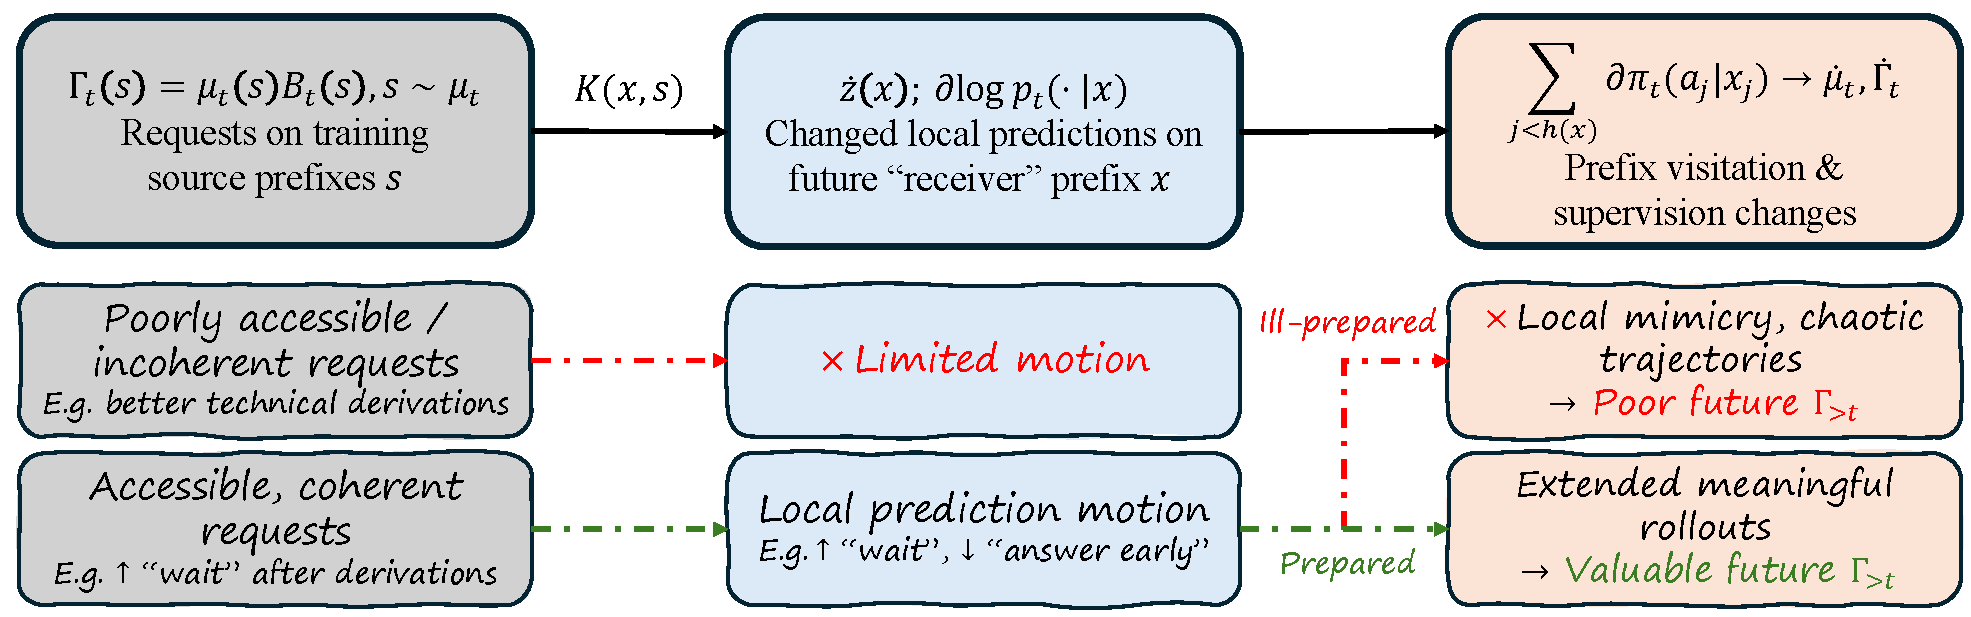
\includegraphics[width=1.0\linewidth]{figures/opd_illustration.pdf}
\caption{OPD's learning dynamics, visualizing the feedback loop at the top (detailed in \Cref{sec:loop}), and illustrative successful and failing processes at the bottom in reasoning settings we analyzed empirically. In principle, OPD propagates current teacher requests $\Gamma_t(s)\vert_{s\sim\mu_t}$ to motion at any future prefix $x$ through shared parameters, captured by the Neural Tangent Kernel $K(x,s)$. Such policy motion shapes how the autoregressive rollout (prefix visitation) and supervision distribution changes ($\dot{\mu}_t, \dot{\Gamma}_t$). In practice, a healthy dynamics needs not only locally ``tangent-accessible'' and coherent requests (\Cref{sec:conversion}), but also the student to be sufficiently ``prepared'', so that it can sustain meaningful rollouts with learning value as it absorbs corrections requested by the teacher, instead of primarily performing local mimicry and falling into chaotic rollouts hard for the teacher to rescue, let alone improve on (\Cref{sec:broadcast,sec:preparation}).}
\label{fig:opd_illustration}
\end{figure}


The dependence of OPD on the student sustaining stable rollouts (prefixes) which induce meaningful supervision motivates offline preparation. Here, the weak student is first forced to visit the teacher's prefixes and learn predictions there, enabling the subsequent OPD process to sustain productive learning as the student exposes finer correction opportunities to the teacher, while maintaining stabler and more recoverable changes in its rollout distribution. Across Qwen-2.5 and Llama-3.1 models on AIME 2024 and 2025 problems, we find that under sufficient offline training, the subsequent OPD phase substantially improve pass@$k$ (for $k$ up to 32) and per-problem reliability compared to offline training alone. In the rest of the paper, we present these results and insights organized under the following three questions. What determines the \emph{conversion} of teacher supervision into policy motion (\Cref{sec:conversion})? Does the \emph{broadcast} of these updates across prefixes improve subsequent reasoning or steer the student toward unreliable continuations and supervision (\Cref{sec:broadcast})? Can offline \emph{preparation} strengthen the student’s continuation ability and enable productive on-policy learning (\ref{sec:preparation})?


\textbf{Related works}. We briefly discuss related works here, and leave the expanded version to Appendix \cref{app:related-work}. \emph{On-policy distillation.} Training on learner-generated states with expert feedback is a classical approach to addressing distribution shift in imitation learning \citep{ross2011reduction}, applied to autoregressive distillation by \citet{lin2020autoregressiveknowledgedistillationimitation}. \citet{gu2023minillm} develop reverse-KL distillation using student rollouts, while \citet{agarwal2024onpolicydistillation} unify on-policy and off-policy training across multiple divergences. \citet{tinker_opd_2025} demonstrate its effectiveness for reasoning and personalization in language-model post-training. More recently, \citet{yang2026gopd} interpret OPD as dense KL-constrained reinforcement learning and introduce reward extrapolation. Empirical studies identify teacher-student compatibility on student prefixes as important factors in transfer and training failure \citep{rethinking_opd_2026,fu2026revisitingonpolicydistillationempirical}.

\emph{Learning dynamics of finetuning.} Kernel-based analyses connect parameter updates to changes in language-model predictions \citep{malladi2023kernelbasedviewlanguagemodel}. \citet{ren2025learning} decompose per-step prediction changes using the loss gradient and empirical tangent kernel, analyzing confidence dynamics in SFT and DPO \citep{rafailov2024directpreferenceoptimizationlanguage}. \citet{tomihari2026rl} study how RL updates propagate across examples, while \citet{shen2026geometryonpolicydistillation} identify persistent low-dimensional subspaces in OPD updates. Building on these perspectives, we connect the student’s evolving tangent kernel to its response to teacher supervision, the quality of its continuations, and the resulting distribution of future training prefixes. This distinguishes limited response to supervision from policy changes that worsen generation, and explains how either can shape subsequent learning.
